%%%%%%%%%%%%%%%%%%%%%%%%%%%%%%%%%%%%%%%%%
% Short Sectioned Assignment
% LaTeX Template
% Version 1.0 (5/5/12)
%
% This template has been downloaded from:
% http://www.LaTeXTemplates.com
%
% Original author:
% Frits Wenneker (http://www.howtotex.com)
%
% License:
% CC BY-NC-SA 3.0 (http://creativecommons.org/licenses/by-nc-sa/3.0/)
%
%%%%%%%%%%%%%%%%%%%%%%%%%%%%%%%%%%%%%%%%%

%----------------------------------------------------------------------------------------
%	PACKAGES AND OTHER DOCUMENT CONFIGURATIONS
%----------------------------------------------------------------------------------------

\documentclass[paper=a4, fontsize=11pt]{scrartcl} % A4 paper and 11pt font size

\usepackage[T1]{fontenc} % Use 8-bit encoding that has 256 glyphs
%\usepackage{fourier} % Use the Adobe Utopia font for the document - comment this line to return to the LaTeX default
\usepackage[english]{babel} % English language/hyphenation
\usepackage{mathtools}
\usepackage{amsfonts,amsthm} % Math packages
\usepackage{wrapfig}
\usepackage{pgfplots}
\usepackage{lipsum} % Used for inserting dummy 'Lorem ipsum' text into the template
\usepackage{hyperref}
\usepackage{url}
\usepackage{numberedblock}
\usepackage{graphicx}
\usepackage{float}
\hypersetup {
    colorlinks=true,       % false: boxed links; true: colored links
    linkcolor=blue,          % color of internal links (change box color with linkbordercolor)
    urlcolor=blue           % color of external links
}

\usepackage{sectsty} % Allows customizing section commands
%\allsectionsfont{\centering \normalfont\scshape} % Make all sections centered, the default font and small caps
\allsectionsfont{\normalfont\scshape}

\usepackage{fancyhdr} % Custom headers and footers
\pagestyle{fancyplain} % Makes all pages in the document conform to the custom headers and footers
\fancyhead{} % No page header - if you want one, create it in the same way as the footers below
\fancyfoot[L]{} % Empty left footer
\fancyfoot[C]{} % Empty center footer
\fancyfoot[R]{\thepage} % Page numbering for right footer
\renewcommand{\headrulewidth}{0pt} % Remove header underlines
\renewcommand{\footrulewidth}{0pt} % Remove footer underlines
\setlength{\headheight}{0pt} % Customize the height of the header

\usepackage{titlesec}% http://ctan.org/pkg/titlesec
\titleformat{\section}%
  [hang]% <shape>
  {\normalfont\bfseries\Large}% <format>
  {}% <label>
  {0pt}% <sep>
  {}% <before code>
\renewcommand{\thesection}{}% Remove section references...
\renewcommand{\thesubsection}{\arabic{subsection}}%... from subsections

%\numberwithin{equation}{section} % Number equations within sections (i.e. 1.1, 1.2, 2.1, 2.2 instead of 1, 2, 3, 4)
\numberwithin{figure}{section} % Number figures within sections (i.e. 1.1, 1.2, 2.1, 2.2 instead of 1, 2, 3, 4)
\numberwithin{table}{section} % Number tables within sections (i.e. 1.1, 1.2, 2.1, 2.2 instead of 1, 2, 3, 4)

\setlength\parindent{0pt} % Removes all indentation from paragraphs - comment this line for an assignment with lots of text

%----------------------------------------------------------------------------------------
%	TITLE SECTION
%----------------------------------------------------------------------------------------

\newcommand{\horrule}[1]{\rule{\linewidth}{#1}} % Create horizontal rule command with 1 argument of height

\title{	
\normalfont \normalsize 
\textsc{CSCI 4360/6360 Data Science II} \\
\textsc{Department of Computer Science} \\
\textsc{University of Georgia} \\ [15pt] % Your university, school and/or department name(s)
\horrule{0.5pt} \\[0.3cm] % Thin top horizontal rule
\huge Assignment 5: Embeddings All The Way Down \\ % The assignment title
\horrule{2pt} \\[0.4cm] % Thick bottom horizontal rule
}

\author{Aditya Shinde} % Your name

%\date{\normalsize\today} % Today's date or a custom date
\date{\normalsize Out October 19, 2017}

\begin{document}

\maketitle % Print the title

%----------------------------------------------------------------------------------------
%	PROBLEM 1
%----------------------------------------------------------------------------------------

\section*{Questions}

This homework assignment focuses on embedding strategies with a touch of neural networks. \\

\textbf{This homework requires more coding than previous assignments, so plan accordingly!} It also does NOT use autograding; whether that's a blessing or curse may vary, but it also means that no example data or code templates will be provided. Furthermore, you'll be asked to generate figures and embed them in your homework write-up.

\setcounter{subsection}{0}

\subsection{Neural Networks \textbf{[25pts]}}

\par A neural network with a single hidden layer and a linear activation will form a linear hypothesis. So it will be able to model a polynomial with degree one very accurately.\\

\par For the hinge loss function, \\

\par Polynomials of degree two cannot be represented by neural networks. These are non linear functions. And with linear activations, we can have only linear hypotheses. \\

\par Piecewise constant functions cannot be represented by linear networks. However, they can be approximated upto a certain degree. for instance a step function which is defined by:

$$
f(x) = \begin{cases}
	1 & x \ge 0 \\
	0 & \textrm{otherwise}
\end{cases}
$$


\begin{tikzpicture}
  \begin{axis}[ 
    xlabel=$x$,
    ylabel={$f(x)$},
    ymin=-3,
    ymax=3
  ] 
    \addplot[-,domain=0:1]{0}; 
    \addplot[-,domain=1:2]{1};
    \addplot[-,domain=2:3]{2}; 
    \addplot[-,domain=3:4]{3};

  \end{axis}
\end{tikzpicture}

This function can be approximated in the following way. \\

\begin{tikzpicture}
  \begin{axis}[ 
    xlabel=$x$,
    ylabel={$f(x)$},
    ymin=-3,
    ymax=3
  ] 
    \addplot[<->,domain=-3:3]{x-0.5}; 
  \end{axis}
\end{tikzpicture}

\par Now this is certainly a very bad approximation. And this particular function is just one from the family of many piecewise constant functions. So the answer would be no. Since not all step functions can be approximated by a linear network. 

Consider the following XOR-like function in two-dimensional space:

$$
f(x_1, x_2) = \begin{cases}
	1 & x_1, x_2 \ge 0 \textrm{or}\ x_1, x_2 < 0 \\
	-1 & \textrm{otherwise}
\end{cases}
$$

We want to represent this function with a neural network. For some reason, we decide we only want to use the threshold activation function for the hidden units and output unit:

$$
h_{\theta}(v) = \begin{cases}
	1 & v \ge \theta \\
	-1 & \textrm{otherwise}
\end{cases}
$$

\textbf{[13pts]} Show that the smallest number of hidden layers needed to represent this XOR function is two. Give a neural network with two hidden layers of threshold functions that represent $f$, the XOR function. Again, you are welcome to provide a drawing, but that drawing must include values being propagated from each neuron. Alternatively, you could draw a table showing the values at each layer.

\subsection{Kernel Smoothing \textbf{[35pts]}}

In this problem, we'll look at nonparametric kernel smoothing for approximating a function from noisy data. We'll also throw in leave-one-out cross-validation to observe its effects on the learned function. For the sake of simplicity, we'll stick with one-dimensional data. \\

We have a ``dataset'' $(x_1, y_1), (x_2, y_2), ..., (x_n, y_n)$, as follows:

$$
y_i = f(x_i) + \epsilon_i
$$

where $\epsilon_i \sim \mathcal{N}(0, \sigma^2)$. \\

The goal of any regression problem is to estimate the true $f(x)$ with an empirical estimate $\hat{f}(x)$. The Nadaraya-Watson estimator is given by:

$$
\hat{f}(x_k) = \frac{\sum_{i = 1}^n y_i K\left( \frac{|x_i - x_k|}{h} \right)}{\sum_{i = 1}^n K \left( \frac{|x_i - x_k|}{h} \right)}
$$

where $K(\cdot)$ is the kernel, and $h$ is the bandwidth. In this example, we'll use the Gaussian kernel:

$$
K(a) = \frac{1}{\sqrt{2 \pi}}  \textrm{exp} \left\{ \frac{-a^2}{2} \right\}
$$

In this equation, $h$ takes the place of the standard deviation, and the data point $x$ will take the place of the mean. \\

(yes: you're going to be writing some code!) \\

\textbf{[5pts]} Write a basic Python program that generates our dataset.

\begin{itemize}
	\item Sample $x_i \sim U(-5, 5)$ (that's a uniform distribution from -5 to 5)
	\item Sample $\epsilon_i \sim \mathcal{N}(0, 0.1)$
	\item Set $y_i = \sin(x_i) + \epsilon_i$
\end{itemize}

\textbf{[3pts]} Implement a squared loss function $\ell(\cdot)$ (you can use vectorized NumPy arrays for this):

$$
\ell(y, \hat{f}(x)) = (y - \hat{f}(x))^2
$$

\textbf{[2pts]} Sample a dataset of size $n = 100$ and plot it; you can use \texttt{matplotlib.pyplot.scatter}). Overlay the scatter plot with the true regression function (meaning compute the $\sin(\cdot)$ of each $x_i$ and plot that in addition to the $y_i$ you computed); you can use \texttt{matplotlib.pyplot.plot}. \\

\textbf{[20pts]} Now, write a program which performs the following:
\begin{itemize}
	\item Sample a ``training set'' of size $n = 100$, and a ``testing set'' of size $m = 100$.
	\item Compute the kernel smoother for a particular choice of $h$, along with the empirical error (average loss between all $y$ and $\hat{f}(x)$), leave-one-out cross-validation error (average loss), and testing error (average loss).
	\item Compute those measurements for the following values of $h \in \\ \{1.0, 0.75, 0.5, 0.25, 0.1, 0.05, 0.01, 0.005, 0.001 \}$.
	\item Construct scatter plots of test error versus empirical error, and test error versus leave-one-out cross-validation error. Test error should always be on the $y$-axis.
	\item Choose the function $\hat{f}$ which minimizes leave-one-out cross-validation error, and plot the training data sample along with the value of this function evaluated on the training data $x$ values.
\end{itemize}

\textbf{[5pts]} Explain why it is a bad idea to merely minimize the empirical risk in problems like this (\emph{HINT:} refer to the last two plots). \\

\textbf{Include your code in a file named \texttt{assignment5\_q2.py} when you submit to AutoLab, as this will be manually inspected. Include the plots in your write-up.}

\subsection{Stochastic SVD \textbf{[40pts]}}

\subsection*{1}
 Implemented as the function compute\_Q(A,k) in the code.\\

\subsection*{2}
 Implemented as the function SSVD(A,Q) in the code.\\

\subsection*{3}

 The plots for the singular values are plotted below. The points in red are the singular values for the SSVD operation for $k=20$ and the ones in blue are the singuler values computed using the deterministic implementation of SVD in scipy. The plots are shown on the next page along with the plots for oversampling.\\


\subsection*{4}
Plots are on the next page along with the plots for the previous question.

\begin{figure}[H]

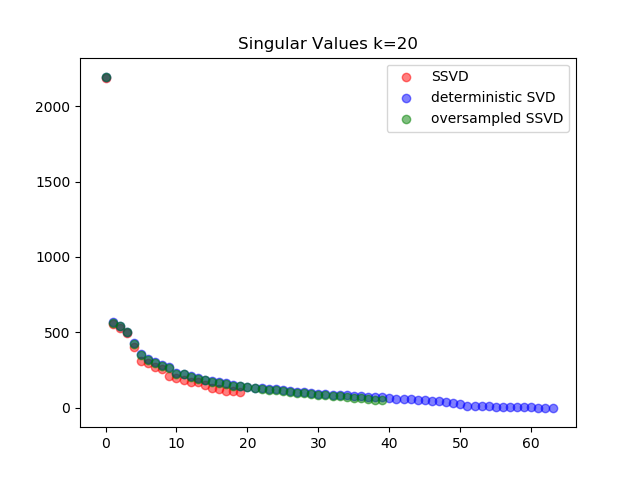
\includegraphics{sing_values_0.png}
\end{figure}

\begin{figure}[H]

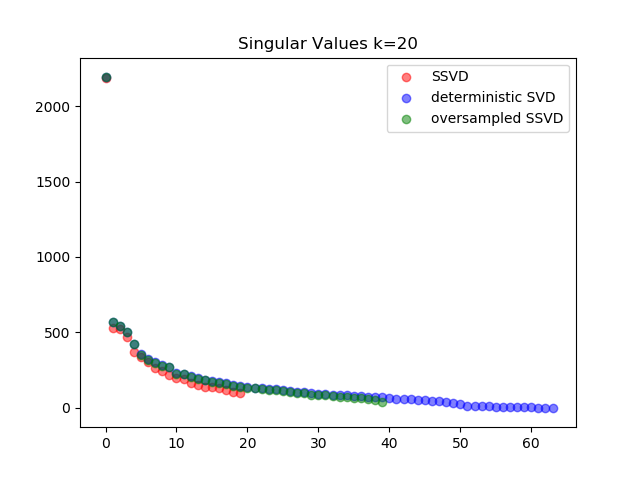
\includegraphics{sing_values_1.png}
\end{figure}

\begin{figure}[H]

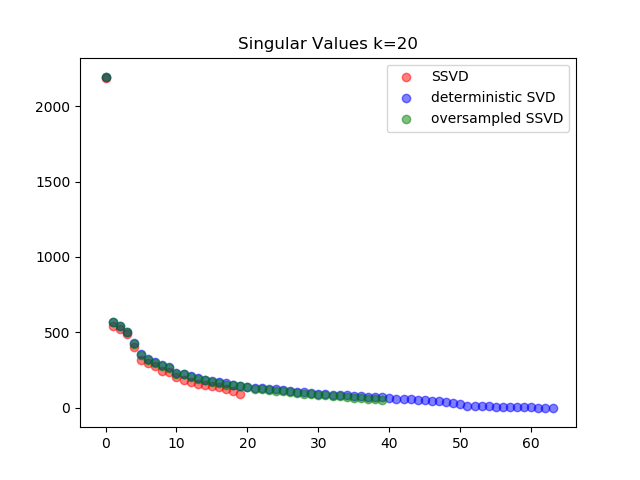
\includegraphics{sing_values_2.png}
\end{figure}

\begin{figure}[H]

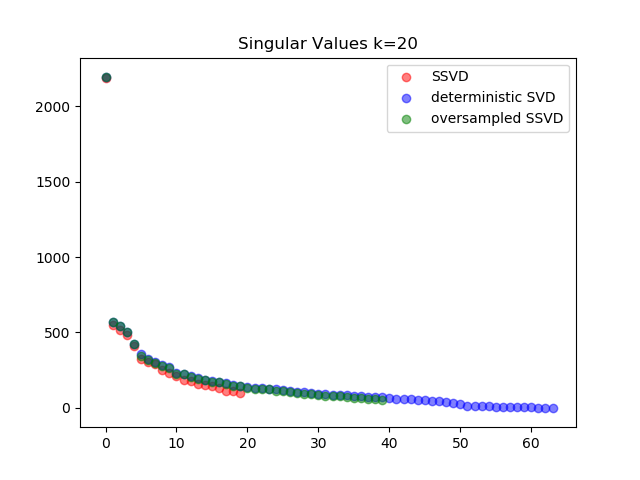
\includegraphics{sing_values_3.png}
\end{figure}

\begin{figure}[H]

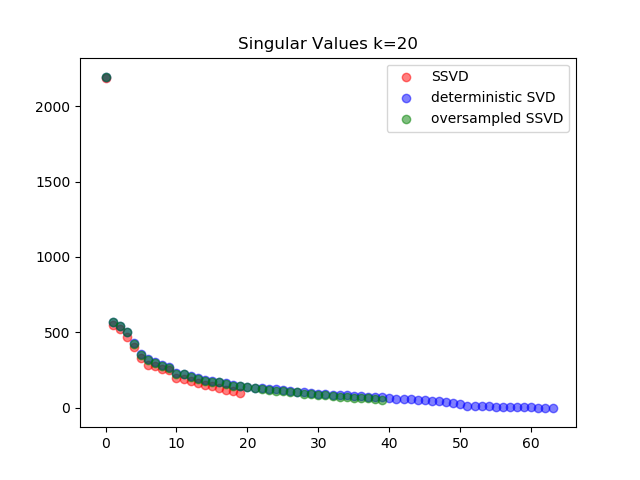
\includegraphics{sing_values_4.png}
\end{figure}

\begin{figure}[H]

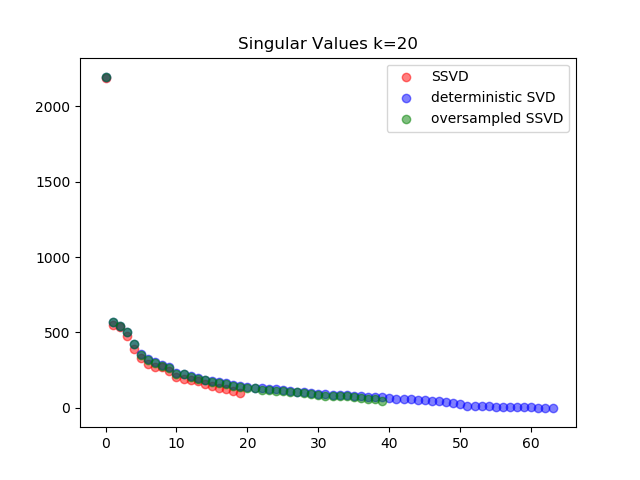
\includegraphics{sing_values_5.png}
\end{figure}

\begin{figure}[H]

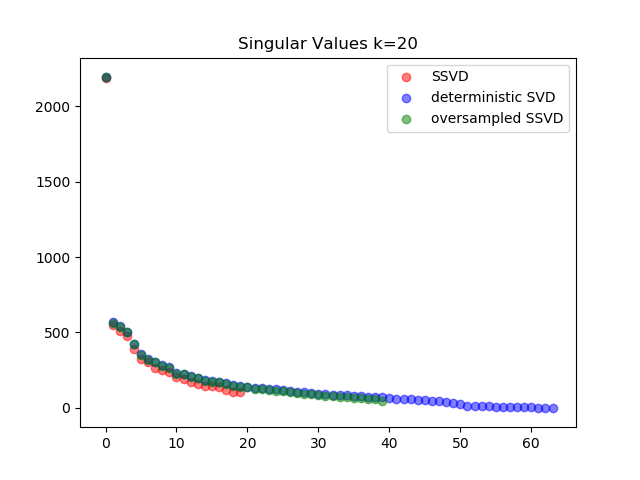
\includegraphics{sing_values_6.png}
\end{figure}

\begin{figure}[H]

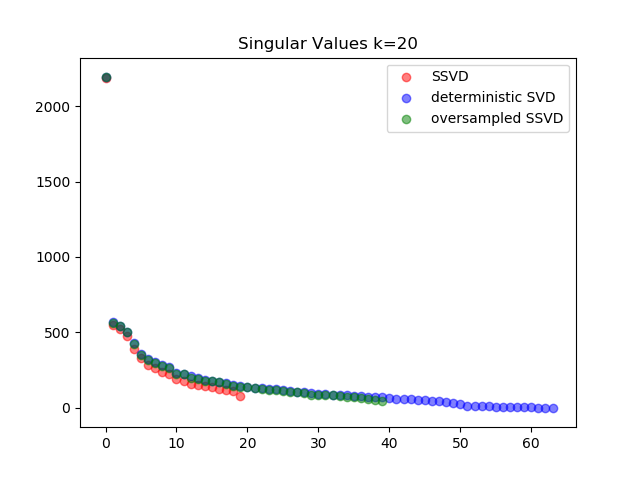
\includegraphics{sing_values_7.png}
\end{figure}

\begin{figure}[H]

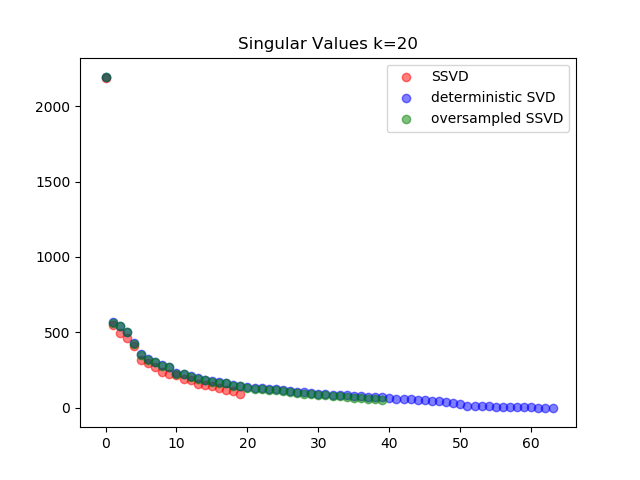
\includegraphics{sing_values_8.png}
\end{figure}

\begin{figure}[H]

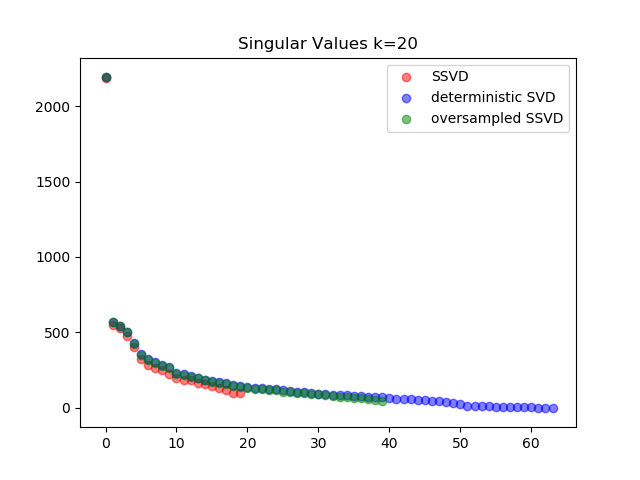
\includegraphics{sing_values_9.png}
\end{figure}

\subsection*{2}


\textbf{BONUS [20pts]} Another way of stabilizing SSVD beyond oversampling is to perform \emph{power iterations} during the orthogonalization step of the preconditioner computations. After computing the initial $Q$ matrix from the QR decomposition, but before applying it to compute $B$, some number of power iterations $q$ are applied to the system to ``refine'' the preconditioner $Q$. \\

Write a Python function that takes an initial $Q_0$ preconditioner, a number of power iterations $q > 0$, and the data matrix $A$. It will return $Q_q$, the preconditioner with $q$ power iterations applied to it. \\

Each power iteration $i$ consists of two discrete steps:
\begin{enumerate}
	\item Form the product $Y = AA^TQ_{i - 1}$
	\item Re-run the QR decomposition to find $Q_i$ using $Y$ from the first step
\end{enumerate}

Re-run your SSVD function on the MNIST data 10 times for $q = 0, 1, 2,$ and 3 respectively (you can also retain the oversampling from before). Plot the singular values and compare them to the built-in SVD solver. How do they stack up? \\

\textbf{BONUS [10pts]} As of \texttt{scikit-learn} version 0.18, Nathan Halko's SSVD solver has actually been integrated! Let's see how your SSVD implementation compares to the ``official'' one. You'll find this implementation if you use \texttt{sklearn.decomposition.PCA} with the \texttt{svd\_solver} parameter set to ``randomized'' in the constructor. \\

Run this solver on the MNIST data, as well as your custom-built SSVD solver, and plot the resulting singular values. How do they compare? What about to a deterministic solver? Is your SSVD better than scikit-learn's? \\

\textbf{BONUS [5pts]} If you implemented power iterations, you can also compare those directly against the one in scikit-learn via the ``iterated\_power'' argument in the constructor (this is essentially $q$). Again, try a few different values of $q$ in your solver and the one in scikit-learn and plot the resulting singular values. How do they look? \\

\textbf{Include your code in a file named \texttt{assignment5\_q3.py} when you submit to AutoLab, as this will be manually inspected. Include the plots in your write-up.} 

\section*{Administration}
\setcounter{subsection}{0}

\subsection{Submitting}

All submissions will go to \textbf{AutoLab}. You can access AutoLab at:

\begin{itemize}
	\item \url{https://autolab.cs.uga.edu}
\end{itemize}
	
You can submit deliverables to the \textbf{Assignment 5} assessment that is open. When you do, you'll submit two files:

\begin{enumerate}
	\item \texttt{\textbf{assignment5\_q2.py}}: the Python script that implements kernel smoothing
	\item \texttt{\textbf{assignment5\_q3.py}}: the Python script that implements SSVD
	\item \texttt{\textbf{assignment5.pdf}}: the PDF write-up with any questions that were asked
\end{enumerate}

These should be packaged together in a tarball; the archive can be named whatever you want when you upload it to AutoLab, but the files in the archive should be named \textbf{exactly} what is above. Deviating from this convention could result in my annoyance! \\

To create the tarball archive to submit, run the following command (on a *nix machine):

\begin{verbatim}
	> tar cvf assignment5.tar *.py assignment5.pdf
\end{verbatim}

This will create a new file, \texttt{assignment5.tar}, which is basically a zip file containing your Python scripts and PDF write-up. Upload the archive to AutoLab. There's no penalty for submitting as many times as you need to, but keep in mind that swamping the server at the last minute may result in your submission being missed; AutoLab is programmed to close submissions \emph{promptly} at 11:59pm on November 2, so give yourself plenty of time! A late submission because the server got hammered at the deadline will \emph{not} be acceptable (there is a \emph{small} grace period to account for unusually high load at deadline, but I strongly recommend you avoid the problem altogether and start early). \\

\subsection{Reminders}

\begin{itemize}
	\item If you run into problems, ping the \texttt{\#questions} room of the Slack chat. If you still run into problems, ask me. But please please please, \textbf{do NOT} ask Google to give you the code you seek! I will be on the lookout for this (and already know some of the most popular venues that might have solutions or partial solutions to the questions here).
	\item Prefabricated solutions (e.g. \texttt{scikit-learn}, OpenCV) are NOT allowed! You have to do the coding yourself! But you \textbf{can} use the various modules mentioned throughout this write-up, so long as they don't replace the required code.
	\item If you collaborate with anyone, just mention their names in a code comment and/or at the top of your homework writeup.
\end{itemize}

\end{document}